\chapter{Proposed System and Design}

This chapter explains the proposed system, studies its feasibility and presents the design of the system with the help of the architecture diagram, use case diagram, data flow diagrams and ER diagram. The project schedule is given at the end of the chapter.

\section{Proposed System}
The proposed system is a cloud based platform that combines IoT, AI, explainable AI and RAG to give farmers reliable and personalised advice. The system is divided into six modules.

\begin{enumerate}
  \item \textbf{Sensor and IoT Module:} Collects real time soil, weather and field data using IoT sensors connected to an ESP32 board.
  \item \textbf{Communication Module:} Transmits the sensor data securely from the edge device to the cloud.
  \item \textbf{AI Recommendation Module:} Recommends suitable crops, fertilizers, irrigation plans and the expected profitability.
  \item \textbf{XAI and RAG Module:} Explains the AI recommendations and provides reliable agricultural guidance from a trusted knowledge base.
  \item \textbf{Database and Dashboard Module:} Stores farm data and displays real time insights through a multilingual interface.
  \item \textbf{User Management Module:} Handles secure registration, login and profile management for farmers and administrators.
\end{enumerate}

The working of the system in brief is as follows. The farmer registers and enters the basic details of the farm. The ESP32 unit sends soil and environment readings to the cloud, where they are cleaned and stored. When the farmer asks for a recommendation, the AI module combines the sensor values with weather data and the farm profile, ranks the crops and finds the fertilizer and irrigation advice. The market module estimates the price and profit of each crop. The XAI module prepares the explanation, and the RAG module can retrieve supporting guidelines from the knowledge base. Finally, the result is shown on the dashboard in the language of the farmer.

\section{Feasibility Study}
\subsection{Technical Feasibility}
The system uses AI/ML algorithms, IoT sensors, weather APIs, cloud computing and web and mobile technologies, all of which are mature and well documented. It can be developed using open source frameworks, publicly available crop datasets and affordable hardware such as the ESP32. Explainable AI libraries and RAG tools such as LangChain and ChromaDB are open source, so the integration of XAI and RAG is also technically possible. Existing research \cite{sharafat2025,sawant2026} has already shown that IoT-based prediction and RAG based advisory work in practice.

\subsection{Operational Feasibility}
The system provides a simple multilingual interface for farmers with different technical backgrounds. It delivers real time crop, fertilizer, irrigation and market recommendations and improves farm decision making. Since manual input is also allowed, a farmer who does not have the sensor unit can still use the system. For administrators, the dashboard makes the management of users, datasets and logs simple.

\subsection{Economic Feasibility}
The project reduces crop losses through accurate crop recommendation and optimises the use of water, fertilizer and other resources. The development cost is low because open source software is used and the field unit is built from low cost components. The cloud services are charged according to usage, so the cost grows only when the number of users grows. The expected savings in inputs and the improvement in productivity and profitability are greater than the cost of the system.

\section{Design}
The design of the system is user centric and modular. The main design diagrams are explained below.

\subsection{Architecture Diagram}

An architecture diagram provides an overall view of the major components of a
software system and the connections between them. The architecture of the
Farming Intelligence AI consists of five main layers, as shown in
Figure~\ref{fig:arch}.

\begin{figure}[H]
  \centering
  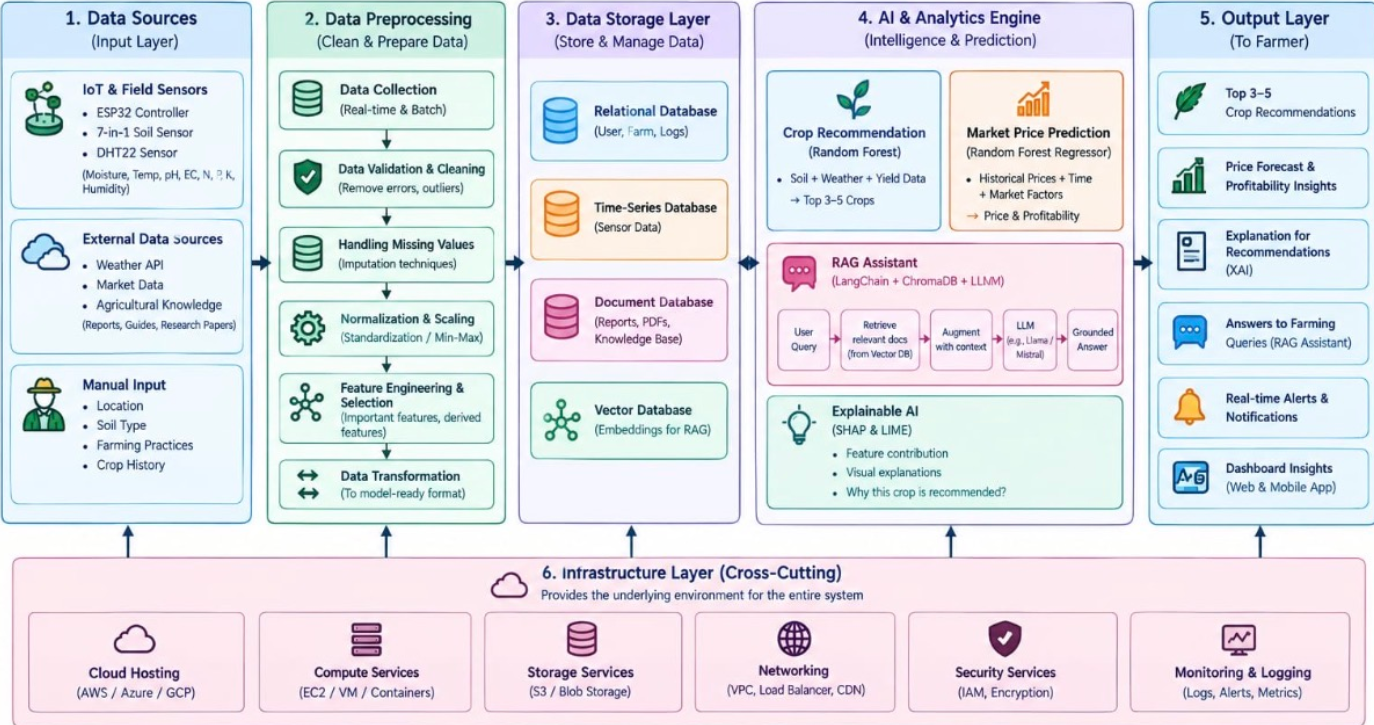
\includegraphics[width=\linewidth]{img/arch.png}
  \caption{Architecture Diagram of the Farming Intelligence AI}
  \label{fig:arch}
\end{figure}

\begin{enumerate}
  \item \textbf{Presentation Layer:} The farmer and the administrator interact
  with the system through a responsive React and TypeScript based web
  application. The layer provides interfaces for farm profile management,
  crop recommendation, explainable AI, fertilizer and irrigation advisory,
  market and profitability analysis, live IoT monitoring, and the
  RAG-based agricultural AI assistant.

  \item \textbf{Application and Backend Layer:} The backend is implemented
  using TypeScript, Node.js and Express. It handles API requests, routing,
  authentication services, IoT telemetry, weather data processing and
  communication between the application components. It also integrates the
  agro-advisory, preprocessing, fertilizer calculation, and market and
  profitability services.

  \item \textbf{AI and Intelligence Layer:} This layer contains the core
  intelligent functionalities of the system, including the crop
  recommendation engine, top crop ranking, explainable AI using SHAP and
  LIME, fertilizer recommendation, irrigation advisory, market and price
  forecasting, profitability analysis, and the RAG-based agricultural AI
  assistant powered by the Gemini API.

  \item \textbf{Data and Storage Layer:} Firebase Authentication is used for
  user and administrator authentication, while Firebase Firestore provides
  NoSQL storage for application data. The system also uses the existing crop
  recommendation and market datasets as data resources. Agricultural
  knowledge documents are used by the RAG component to provide
  knowledge-based assistance.

  \item \textbf{Data Integration Layer:} This layer connects the application
  with the ESP32-WROOM-32E and the 7-in-1 Modbus RTU soil sensor for live
  soil measurements, including nitrogen, phosphorus, potassium, pH, moisture,
  temperature and electrical conductivity. It also connects with the
  Open-Meteo weather API and the agricultural datasets used by the system.
\end{enumerate}
\subsubsection{Use Case Diagram}

The use case diagram illustrates the main functionalities of the Farming Intelligence AI system and the interactions of its two primary actors, the farmer and the administrator. The farmer can register or log in to the system, enter farm and soil details, obtain top crop recommendations based on soil and environmental conditions, view XAI explanations to understand the factors influencing the recommendations, and access market and profitability analysis to support crop-selection decisions. The farmer can also interact with the RAG-based AI assistant to obtain relevant agricultural information and guidance. The administrator can securely log in, manage datasets, monitor system logs, and manage registered users.
\begin{figure}[H]
  \centering
  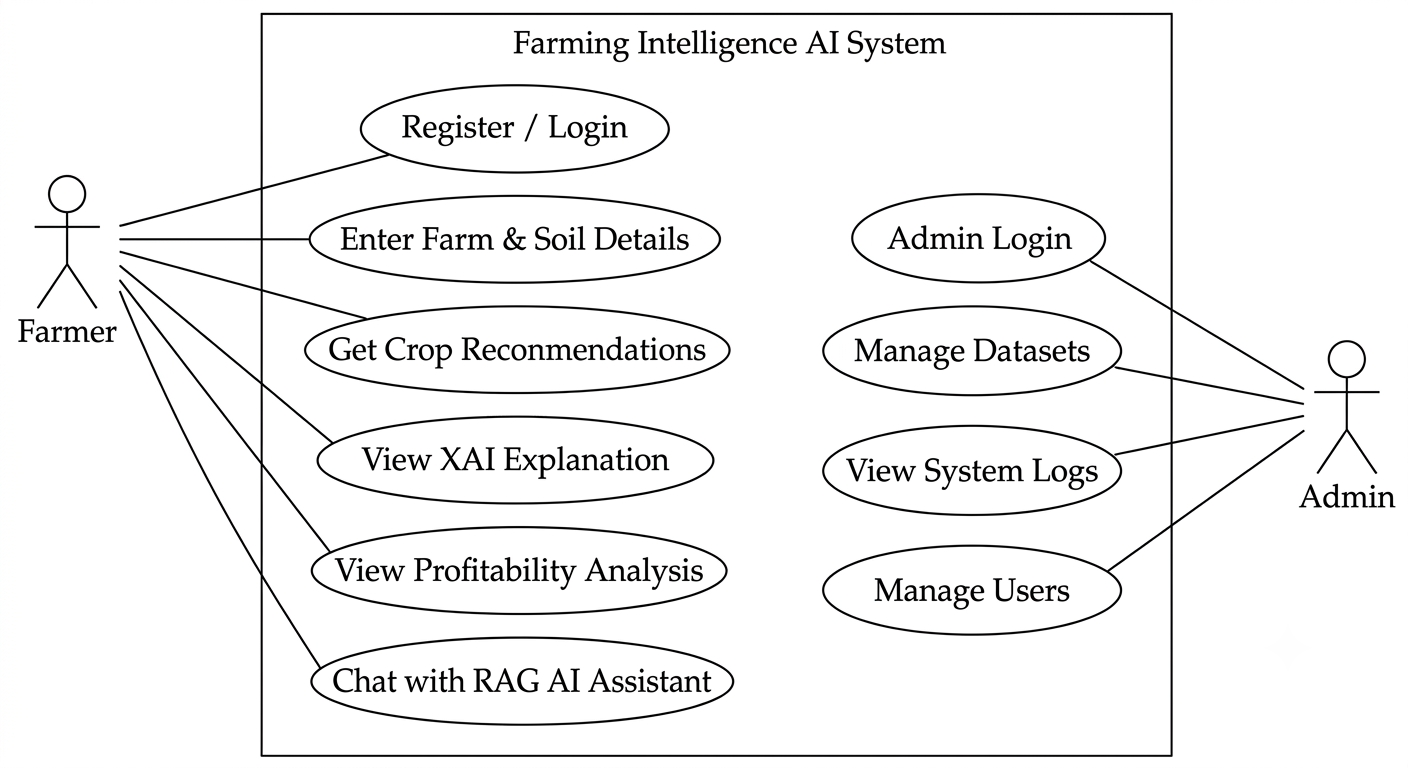
\includegraphics[width=0.90\linewidth]{img/usecase.png}
  \caption{Use Case Diagram}
  \label{fig:dfd0}
\end{figure}

\subsubsection{Level 0 DFD}

Level 0 represents the complete Farming Intelligence AI System as a single process, as shown in Figure~\ref{fig:dfd0}. The external entities are the IoT device, Open-Meteo Weather API and the farmer. The IoT device provides live sensor data to the system, including soil moisture, temperature, humidity, rainfall and NPK values. The Open-Meteo Weather API provides the required weather data for agricultural analysis. The system processes these inputs and generates a personalized farming advisory for the farmer. The advisory includes crop recommendations and other relevant agricultural guidance generated by the system.

\begin{figure}[H]
  \centering
  \includegraphics[width=0.85\linewidth]{img/dfd_level0.png}
  \caption{Data Flow Diagram -- Level 0}
  \label{fig:dfd0}
\end{figure}


\subsubsection{Level 1 DFD}

Level 1 decomposes the Farming Intelligence AI System into six major processes, as shown in Figure~\ref{fig:dfd1}:

\begin{itemize}
  \item \textbf{1.0 Collect and Pre-process Data:} receives live sensor data from the IoT device and weather data from the Open-Meteo weather service. The process validates, combines and prepares the input data for further analysis.

  \item \textbf{2.0 Crop Recommendation:} uses the processed environmental and soil parameters together with the trained 22-crop recommendation dataset to generate suitable crop recommendations and select the top 3--5 recommended crops.

  \item \textbf{3.0 XAI and Advisory Generation:} generates explanations for the recommended crops using XAI techniques such as SHAP/LIME and prepares the agricultural advisory based on the recommendation results.

  \item \textbf{4.0 Market and Profitability Analysis:} uses available market data to analyse crop prices, market trends and profitability for the recommended crops.

  \item \textbf{5.0 RAG Knowledge Retrieval:} retrieves relevant agricultural information from the project knowledge base using the RAG-based retrieval system and provides supporting knowledge for the advisory.

  \item \textbf{6.0 Generate Final Advisory:} combines the crop recommendations, XAI explanation, market and profitability information, fertilizer and irrigation advisory, and relevant knowledge retrieved through RAG to generate the final personalized agricultural advisory for the farmer.
\end{itemize}

\begin{figure}[H]
  \centering
  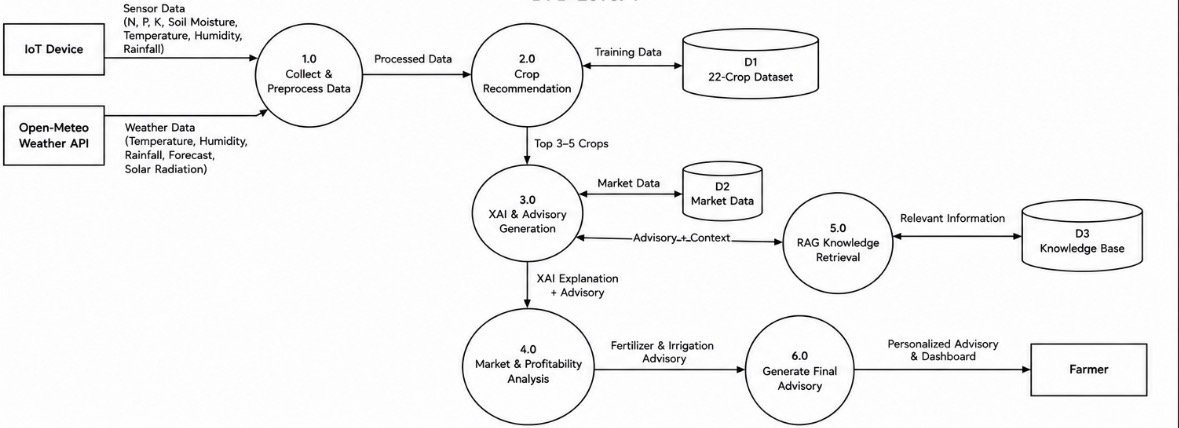
\includegraphics[height=0.2\textheight]{img/dfd_level1.png}
  \caption{Data Flow Diagram -- Level 1}
  \label{fig:dfd1}
\end{figure}

\subsection{ER Diagram}

The ER diagram represents the main entities of the Farming Intelligence AI
system and their relationships, as shown in Figure~\ref{fig:er}. It includes
user details, soil and weather data, crop recommendations, XAI explanations,
agro-advisory, market analysis, AI chat, and system logs.

\begin{figure}[H]
    \centering
    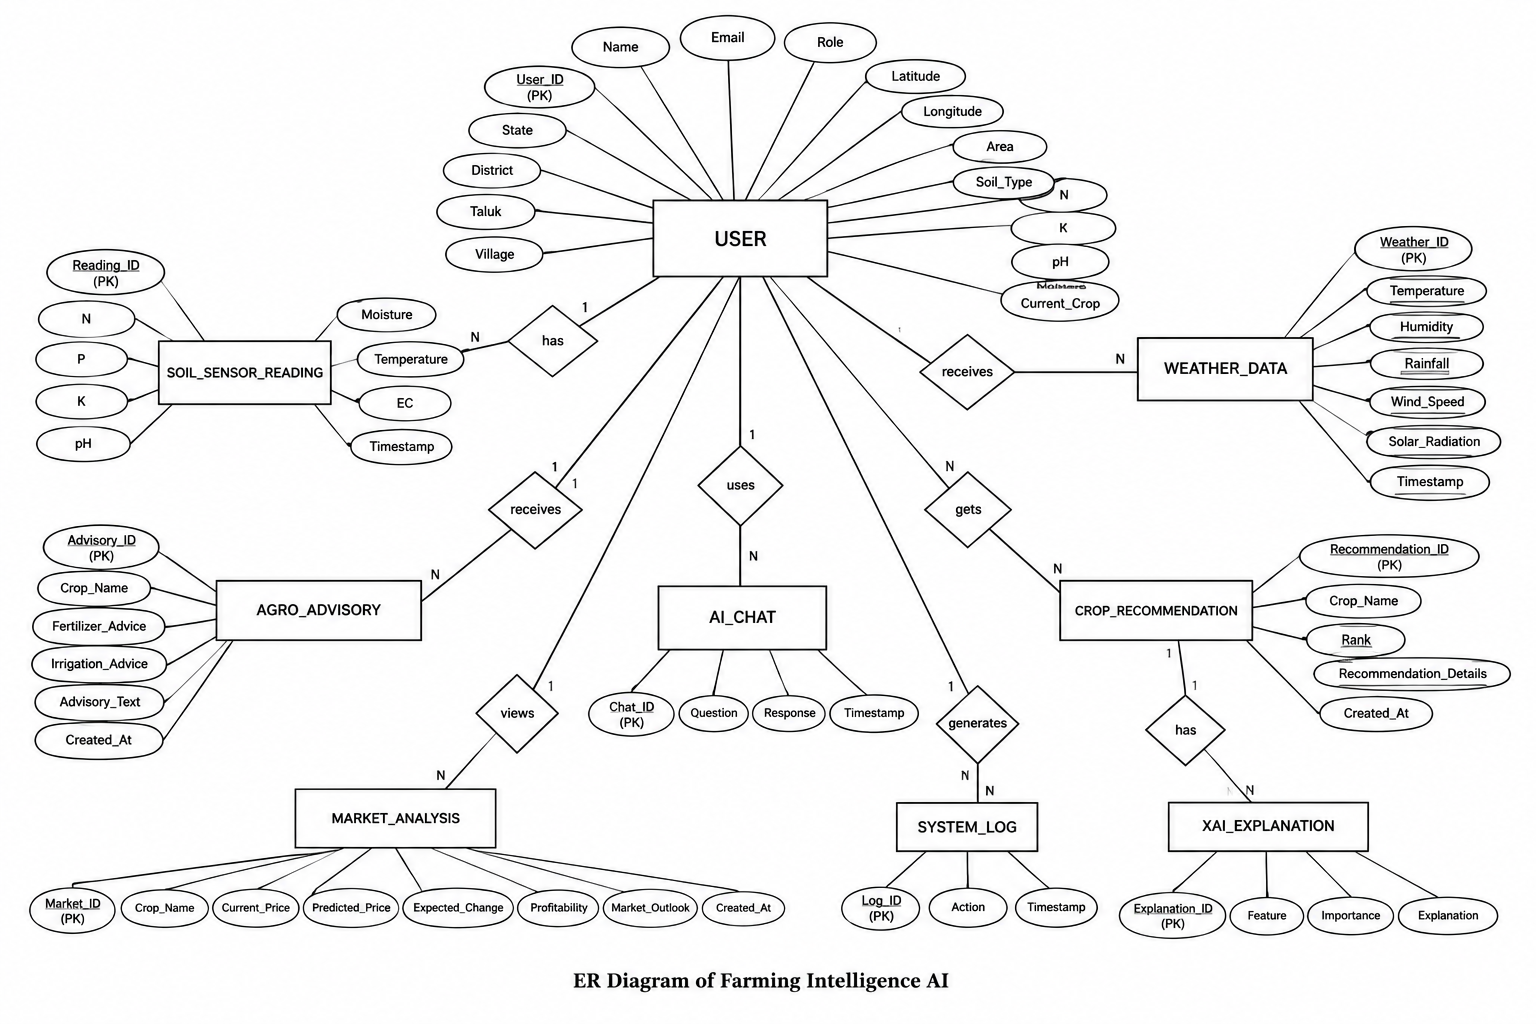
\includegraphics[width=0.98\textwidth]{img/er.png}
    \caption{ER Diagram of the Farming Intelligence AI}
    \label{fig:er}
\end{figure}

The diagram provides a logical representation of the application's data
structure, with Firebase Firestore used as the underlying NoSQL database.

\subsection{Methods and Techniques}

The Farming Intelligence AI integrates various methods and techniques to support
farmers in making informed agricultural decisions. The system combines IoT-based
soil monitoring, weather data analysis, machine learning-based crop
recommendation, explainable AI, fertilizer and irrigation advisory, market
analysis, and a RAG-based agricultural assistant. These techniques work
together to provide personalized and data-driven farming recommendations.

\subsubsection{IoT-Based Soil Monitoring}

The system collects real-time soil parameters using an ESP32-WROOM-32E connected
to a 7-in-1 Modbus RTU soil sensor. The sensor provides nitrogen, phosphorus,
potassium, pH, moisture, temperature, and electrical conductivity values. These
readings are processed and used by the application for agricultural analysis.

\subsubsection{Weather Data Analysis}

Weather information is obtained using the Open-Meteo API. Parameters such as
temperature, humidity, rainfall, and solar radiation are used along with soil
and farm information to support crop recommendation and agricultural advisory.

\subsubsection{Crop Recommendation}

The system uses a machine learning-based crop recommendation approach to
identify suitable crops based on soil and environmental parameters. The model
processes features such as N, P, K, temperature, humidity, pH, and rainfall and
provides a ranked list of suitable crops.

\subsubsection{Explainable AI}

Explainable AI techniques such as SHAP and LIME are used to explain the factors
influencing the crop recommendations. This helps farmers understand which soil
and environmental features contributed to the predicted crops.

\subsubsection{Fertilizer and Irrigation Advisory}

The agro-advisory component provides fertilizer and irrigation recommendations
based on the available soil, weather, and crop information. This helps farmers
make appropriate decisions regarding nutrient management and water usage.

\subsubsection{Market and Profitability Analysis}

The system analyzes available market and price data to provide current price,
predicted price, expected change, market outlook, and profitability information.
This helps farmers evaluate the potential economic benefits of different crops.

\subsubsection{RAG-Based Agricultural Assistance}

The RAG-based AI assistant uses agricultural knowledge documents to provide
context-aware answers to farmers' queries. Relevant information is retrieved
from the available knowledge resources and used with the Gemini API to generate
useful agricultural guidance.